\documentclass[titlepage]{article}

\usepackage{graphicx}
\usepackage{hyperref}
\usepackage{indentfirst}
\usepackage{lipsum}
\usepackage{xcolor}

\begin{document}

	\thispagestyle{empty}
	\topskip0pt
	\vspace*{\fill}
		~\centerline{\textcolor{red}{\Huge{WORK IN PROGRESS}}}
		\newline\newline

		\large{Known Issues}
		\begin{itemize}
			\item Adobe renders the 2.2 (The Parser) AST images oddly unless zoomed in.
		\end{itemize}
	\vspace*{\fill}
	\newpage

	\title{Exploring Best Practices for the Creation of a Programming Language Ecosystem: A Case Study with ProtoSQL}
	\author{Brandon Browning}
	\maketitle

	\begin{abstract}

		Developing a programming language is a process full of managing many different forms of complexity.  This project is an experiment in managing the problems that may arise in the development of an ecosystem for a new programming language; it is meant to explore and evaluate the best practices through the creation of a full language.  This will result in an industrial-strength and full-featured tool chain, including a parser, optimizer, and compiler.  The parser will adhere to the language grammar, generate descriptive error messages, and supply an Abstract Syntax Tree (AST) to the optimizer.  The optimizer will then go through the tree and rewrite pieces as it sees fit, generally to improve performance.  Then the compiler, here a cross-compiler, will take the AST and output corresponding SQL code.

	\end{abstract}

	\section{Insight}

		This project started out with a deep curiosity into how languages are defined, and how people manage the tooling around them.  To somebody who is unfamiliar with workings of parsers and compilers, it seems like such an immense and magical process to have code that turns code into code.  It's always a bit magical, but I hope through this paper to show how the field of Computer Science has dealt with this problem, and why it's not as painful as one would think.

		First I'll go over some of the ideas behind programming languages; such as why new ones should be created, the ecosystem surrounding them, and how different ways they're implemented.  Then I'll describe the process behind the creation of ProtoSQL; including the difficulties faced, the benefits of some of the practices employed, and the overall experience and outcome of working on a new programming language.

	\section{Overview of Creating a New Language}

		Languages are usually created because there's some kind of problem one would like to solve; such as wanting to work at an abstraction level between two other languages, or a completely different way of thinking to some established standard.  Over time, the strengths and weaknesses of a language begin to show.  The weaknesses are not necessarily oversights by the original designer, but more intricacies that are brought out over time by heavy usage of the language.  Due to this phenomenon, the development of new languages serves an important role in the evolution of software.

		\subsection{The Grammar}

			The first part of the process towards the foundation of a new programming language, almost out of necessity, is to develop the syntax and semantics of how the language will function.  There's an already existing domain of problem that the creator wants to solve, so they must think on the constructs used to solve that problem, and how they will fit together.  For example, if somebody wanted to create a language for a hand-held algebra system, they'd have to consider brevity and ease of entry as design goals.  They may opt to limit the feature set and complexity of the language as it's probably aimed at beginners, and the limited input versus a desktop-based system would be a significant factor.  At this point, many of the details aren't known, but the high-level design starts coming in to play which heavily dictates the initial direction of the language.



		\subsection{The Parser}

			Usually the first part of a new programming language ecosystem to be implemented is the parser.  The construction of a parser helps solidify the correctness of the grammar, lets you start working on and provides a basis for the compiler, and helps iron out and explore the grammar.  If the language hasn't been carefully scoured over before work on the parser begins, then problems in the grammar naturally surface during work on the parser.

			Now what exactly does the parser do?  The parser is the engine that turns the source text, or the source material for the entire process, into a structure fed through the rest of the system until completion; this structure is known as an Abstract Syntax Tree (AST).  The AST is a representation of the grammar in the form of a manipulatable data structure.  The primary purpose of the parser is then to turn the source text into its corresponding AST.

			The AST could be visualized as a tree or graph data structure which is common in Computer Science, and where the name comes from; however, this is beyond the scope of the paper.  Essentially, It is a hierarchal structure of the pieces of the language that the source text demonstrates.  For example, here's a simple arithmetic expression:
			\newline

			~\centerline{\Large{$x + 5$}}
			\newline

			This could be represented graphically, slightly simplified, as the following..
			\footnote{AST Graphics generated from \href{http://www.gliffy.com}{gliffy.com} and manipulated with \href{http://www.getpaint.net/}{Paint.NET}}
			\newline

			~\centerline{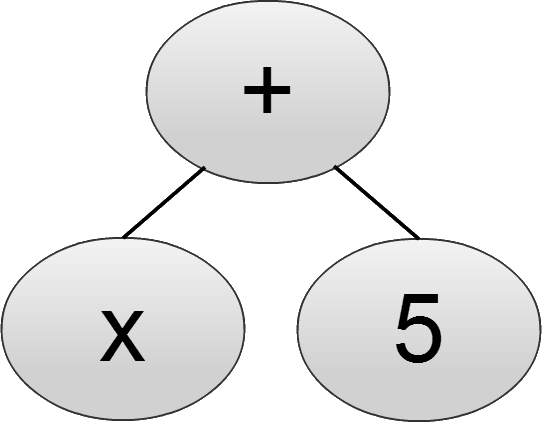
\includegraphics[scale=.3]{ExampleSimpleAST.png}}
			\newline

			A more complex programming-language type expression might be:
			\newline

			~\centerline{\Large{$printf(''(\%d, \%d)'', x, \frac{1}{2})$}}
			\newline

			An AST that's much more similar to how the above expression would be treated in an industrial-strength parser would resemble the following..
			\newline

			~\centerline{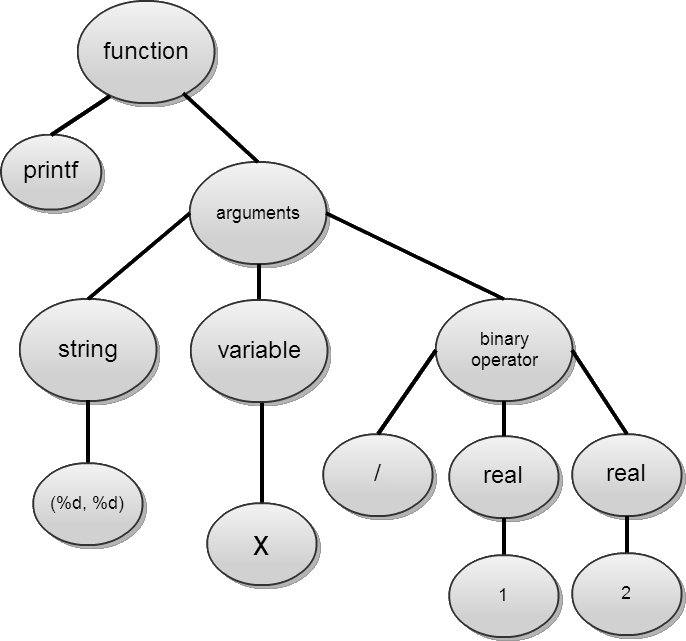
\includegraphics[scale=.5]{ExampleCodeAST.png}}
			\newline

			Here, many of the important details left out of the previous graphic are shown.  The above AST does not have any information as to what plus, x, and 5 are.  Here, we see that at the highest level is a function being called, named printf, which has three arguments.  The type of the argument, as well as its value, are recorded.  Having the tree structure this way makes it quite easy to make optimizations.

			There's two main types of parser implementations; parser generators and less common parser combinators.  Parser generators convert a description of the grammar in a special format, mixed in with pieces of logic, into a new program which parses that grammar.  Parser generators are some of the first parsers made, and produce quite efficient code; however, there is an extra layer of indirection in producing the parser, and the input source code is generally a superset of the language the logic is written in.

			On the other hand, parser combinators are less often used, partially to being relatively new.  They contrast from parser generators by just being a library used to write your parser, not a proprietary extension, and there is no extra step of generating the parser; the code is the parser.  Parser combinators work differently from parser generators by building up large parsers from little parsers.  For example, one may create the functionality to turn any parser into a new parser that parsers a comma-separated list of the original parser.  So given a parser that can parse a number, for example:
			\newline

			~\centerline{$-42.3$}
			\newline

			the new parser will parse:
			\newline

			~\centerline{$-1, 13, 15.6, -.1$}
			\newline

			Then, given another function that parses the input parser surrounded by square brackets, you could generate a new parser resembling:
			\newline

			~\centerline{bracket(comma-seperated(bracket(comma-seperated(parse-number))))}
			\newline

			Which could parse the following:
			\newline

			~\centerline{$[[1, 2], [-1, 42.5], [1]]$}
			\newline

			Creating this parser took almost no effort, and as a bonus, all of the intermediate parsers are available to us.  This way, building up a parser for your grammar allows you to, for free, get all of the parsers you create on the way.  Everything is defined in a composable way, and it's exciting to put together mini-parsers to create a large system.

		\subsection{The Optimizer}

			Optimizers exist to improve the performance of the output.  Generally, a programming language is devised to address difficulties in other languages, and also to provide abstraction; optimizers are an important part in both roles; they can be smarter than previous languages, allowing some of the pains previously endured creating the old language's programs to disappear, and also to allow new abstractions to not come at a high cost.

			The optimizer would be a tool that transformers the AST generated by a parser into a more performant, similar AST, that should effectively behave exactly the same.  For example, the optimizer may crawl down the tree and find the addition operator being used on two constants.  For example:
			\newline

			~\centerline{$delay = duration() * 60 * 1000$}
			\newline

			Here, it may optimize away the addition and replace it with the only result possible, also known as inlining.  The new source may then have this line instead:
			\newline

			~\centerline{$delay = duration() * 60000$}
			\newline

			This is obviously quite a simple optimization, but it's easy to show and understand how the behavior of the program shouldn't differ from the previous version.  Optimizations like this, but much more complex, can save many fold of a program's execution time.

		\subsection{The Compiler}

			The role of the compiler is to translate the optimized AST into the target.  The target of a compiler is usually another language, whether it be one of the same abstraction level, or something much more low-level.  It does this by going through the AST, and deciding how it should be outputted.  Usually this is a recursive process, which when completed leads the the final output and end goal of the programming language; to end up in some other form.  Note the entire process from parsing through compilation is sometimes just known as compiling.

			For example, there may be a compilation system for converting an arithmetic expression from infix to postfix.  This problem could be solved by defining a grammar for infix arithmetic, then parsing it into an AST, and then traversing it in a way that will put the operations in post order.  Given an expression, such as:
			\newline

			~\centerline{\Large{$1 + \frac{5}{3}$}}
			\newline

			This could be represented as the following AST:
			\newline

			~\centerline{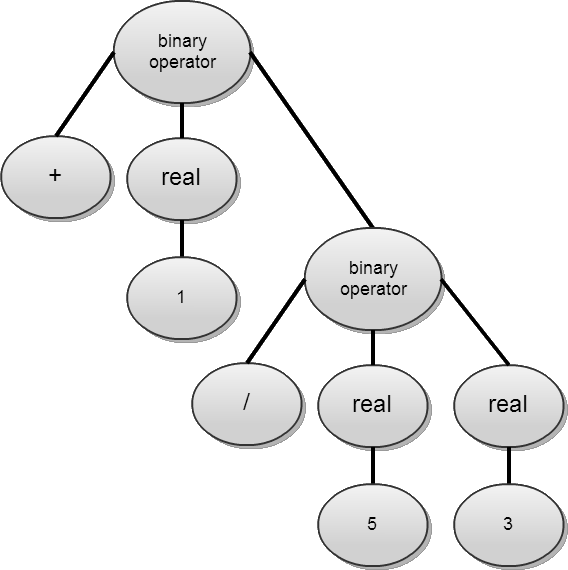
\includegraphics[scale=.5]{ExampleCompileBinaryAST.png}}
			\newline

			The compiler could then recursively traverse down the tree.  If it encounters a real number, it will just output it.  If it encounters a binary operator, however, it will recursively output its children, and then the operator name.  Here's a listing of how this process would occur:
			\newline

			Steps
			\begin{enumerate}
				\itemsep0em
				\item $compile(1 + \frac{5}{3})$
				\item $compile(1)\ compile(\frac{5}{3})\ +$
				\item $1\ (compile(5)\ compile(3)\ /)\ +$
				\item $1\ 5\ 3\ /\ +$
				\newline
			\end{enumerate}

	\section{Implementation of ProtoSQL}

		ProtoSQL began as a combination of two things; a curiosity into the inner-workings of programming languages, and a desire to find an alternative to SQL.  I've never worked on designing or implementing a language, so it's understandable why I didn't know how programming languages work.  However they're an extremely important part of the ecosystem, and I wanted to explore the way they transform text, make smart decisions, and translate it into another domain.  My desire to explore alternatives to SQL comes from a productivity point-of-view, not necessarily from a disagreement with its design; SQL is an old language, and I thought there'd be some ways to make development with it less painful.  It does, however, do its job very well; it just is quite unwieldy and verbose.

		\subsection{The Grammar}

			

\end{document}